%!TEX root = knowledge-curation.tex
\section{Background}
\label{cha:background}
    % What I pretend with this part without title is to provide a non detailed introduction to all the rest of the chapter that put in context the reader. 
    % about the evolution of the channels and the ine
%   Prior to the 21st century, books and classrooms were the main way to learn new programming languages and to answer questions.
%   Software development was an activity performed by small geographically co-located groups using email and phone calls as the main way to coordinate activities, ask questions, collaborate with others, and share knowledge~\cite{Storey2014}.

    The emergence of new \textit{media channels} (e.g., wikis, forums, and Q\&A websites) and \textit{communities of practice} have caused a stir in the industry.
    Project-related activities are scattered among many channels like bug trackers, wikis, and source code repositories~\cite{Guzzi2013}.
    Learning new programming languages is a just-in-time activity performed with the help of online resources~\cite{Sim2013,Storey2010,Hartmann2008}.
    Many projects are now global and open to the public through online repositories, collaboration is not limited by geographical barriers, and a new type of programmer has emerged: \textit{the social programmer}.

    Awareness is one of the main issues that social programmers face on a daily basis.
    The variety of channels available imposes the social programmer to use multiple channels in unison~\cite{Storey2010, Storey2014}.
    Regardless of how social programmers select their preferred channels, they have to invest time in learning the way each channel works.
    Also, channels are becoming increasingly complex with more options for communicating, making media literacy a complex issue.
    %information is available everywhere but the quality of it is also a concern that the social programmer have to deal with.

    The research community have identified various aspects of media channels within communities of practice.
    We have algorithms to detect experts on social channels~\cite{Pal2011a,Pal2012a}, models that explain the propagation of information through channels~\cite{Jin2013, Jiang2013}, an understanding of the relationships between the evolution of the community and its products~\cite{German2013}, and discovered ways that social programmers are using media channels~\cite{Sowe2008a, Singh2009, Parnin2013}.

    Some issues are still pending.
    Issues that current programmers need to understand, including the synergy between media channels and the way these channels affect communities of practices.
    To our knowledge, just a few researchers have investigated these topics.
    We know the activities in mailing lists are correlated to activities in the source code~\cite{Bird2006}, the role of social media in software engineering~\cite{Storey2014, Storey2010}, a complementary perspective on using APIs and the questions asked on Stack Overflow~\cite{Kavaler2013}, and the interplay between Stack Overflow and the software development process, reflected on changes committed in a source code management system~\cite{Vasilescu2013a}.

\subsection{Media channels}

    % What is a media channel?
    The Oxford dictionary\footnote{\url{http://oxforddictionaries.com/definition/english}} defines medium as \textit{``a mean by which something is communicated or expressed''}, and a channel as \textit{``a method or system for communication or distribution''}.
    Combined, a media channel is \textit{``a method or system by which information is communicated or distributed to others using different means''}.

    A media channel is composed of users, messages, and a channel.
    \textit{Users} are the active part and are responsible for the creation of messages.
    \textit{Messages} contain the knowledge transmitted to the receiver and take different forms depending on the channel's characteristics (text, graphics, video, sound, or a combination of them).
    A \textit{channel} provides a method or system to coordinate, communicate, collaborate and share knowledge with other users~\cite{Storey2014}.

Depending on the characteristics of a channel, some tasks are easier to accomplish than others.
For instance, Stack Overflow is changing the way in which developers learn, communicate, collaborate, and share knowledge among themselves~\cite{Storey2014}.
Stack Overflow may even replace the mailing list usage as a consequence of its gamification system, rich interface, and social media features~\cite{Vasilescu2014b}.

%   Some research have focused on different components and aspects of channels, such as,
%categorize questions according to their topic~\cite{Treude2011}, determine the characteristics of unanswered questions~\cite{Asaduzzaman2013}, study the way messages are disseminated on social coding sites~\cite{Jiang2013}, and propose a method to quantify the risk of not having maintainers for code implemented in a certain programming language~\cite{Vasilescu2013b}.

\subsection{Community of practice}
    % What it is
    A community of practice is \textit{``a group of people who share a concern or a passion for something they do and learn how to do it better as they interact regularly''}~\cite{Wenger2000}.
    In contrast with formal work groups and project teams, community members are part of the community by their own will~\cite{Wenger2000}.
    Members work towards a common objective, learning and helping each other in the process.

    % Components
    The core components of a community of practice are the domain, the practice, and the community~\cite{Wenger2011}.
    The \textit{domain}, or shared interest, defines the identity of the community.
    The \textit{practice} identifies members of a community as \textit{practitioners} that are constantly developing and sharing a set of resources (tools, documentation, histories, or experiences) to address recurring problems. 
    The \textit{community}, comprises the activities in which members discuss to help each other, enabling them to learn from the community.

    % Why are they important
    A community of practice is more than the sum of its parts.
    It helps members to solve problems quickly, transfer best practices, develop professional skills, identify experts, form social bounds between members, and drive strategies~\cite{Wenger2011, Storey2014}.
    It also accumulates and updates knowledge through practitioners~\cite{Wenger2010}, enabling them to take a collective responsibility for managing the knowledge according to their needs~\cite{Wenger2011}.
    Given the proper structure, practitioners can be the best option to manage the construction of knowledge~\cite{Wenger2011}.

    % How they change
%   Communities of practice are like living organisms, evolving and adapting according to their context, producing new tools for the community, and external sites.
%   Communities change their practices and structure regularly while adapting dynamically to new situations.
%   For example, Mozilla adopted the Mercurial tool~\cite{Rodriguez-Bustos2012} and changed their version release strategy~\cite{Khomh2012} as a way to keep up with a fast changing business environment.

\subsection{The R community}

The R project\footnote{\url{https://www.r-project.org/}} was born in 1993, as a Free and Open Source programming language and software environment for statistical computing, bioinformatics, and graphics~\cite{Ihaka1996}.
%R is an implementation of the S programming language combined with lexical scoping inspired by Scheme.
%   It was created by Ross Ihaka and Robert Gentleman and is now developed by the R Development Core Team.
The R community is composed of two groups:
\begin{enumerate*}[label=(\arabic*)]
  \item \textit{R-core}, a team of 20 software developers that maintains and evolves the R language, and
  \item \textit{Periphery} includes everybody else (language users and package developers).
\end{enumerate*}

    The R community is an eclectic open source community beyond software development.
    % It provides broader relevance outside the software development community, since it
    It includes biologists and statisticians, with no or limited programming experience.
    Its entire history of mailing list communication is archived and publicly available.
    The R community has also been the subject of extensive research in community evolution~\cite{German2013} and the interplay between channels~\cite{Vasilescu2014c}.

    In our study, we focused the analysis on the R-help mailing list and Stack Overflow, both channels are among the main ones in the R community.
%   As media channels, the R-help mailing list and Stack Overflow provide similar benefits to the R community (i.e., Stack Overflow\footnote{\url{http://stackoverflow.com/tour}} and R-help\footnote{\url{https://www.r-project.org/mail.html}}).
%   The R-help mailing list and Stack Overflow are one of the many channels available within the R community.
    We chose them because their description are similar in terms of the community support.

\subsubsection{R-help Mailing List}
    The R community has a group of mailing lists for helping community members to solve programming problems with R language: \emph{R-help}, \emph{R-package-devel}, \emph{R-devel}, \emph{R-packages}, and \emph{Bioconductor}.
%   Through email, R users can send their questions to different mailing lists depending on the topic.
%   Members subscribed to the R mailing lists can contribute by answering the user directly or posting to the list.
%   In the last case, the email subject is kept as an identifier for the reader.

In particular, the R-help mailing list is to discuss problems and solutions using R. 
Other messages are also encouraged, such as documentation, benchmarks, examples, and announcements not covered by \emph{R-announce} or \emph{R-packages}.
It is oriented to users interested in R, but not necessarily with programming skills.
%   As a mailing list, R-help does not provide a user interface to manage the email threads.

    The R-help mailing list used to be the main media channel for asking and answering questions within the R community, but a significant number of users migrated to Stack Overflow~\cite{Vasilescu2014c}.
    Despite the reduced number of users, the R-help mailing list is still very active; on average, a subscriber may receive 55 emails a day.

\subsubsection{Stack Overflow}
\label{subsec:Rtag}

    In contrast to the R-help mailing list, Stack Overflow incorporates a rich visual and user-friendly interface with social media and gamification features.
    The social aspect of the website improves participation and provides strong support for creating and sharing knowledge as well as encouraging informal mentorship~\cite{Jenkins2009, Storey2014}.
    Meanwhile, gamification provides a system based on reputation points and badges to reward users' participation, thus earning points that enable functionality inside the site.
%   For example, 20 points allow users to participate in the site's chat rooms, 100 points allow users to edit wiki posts, 2000 points allow users to edit questions and answers, and with 25000 points, users can access site analytics.
%   Stack Overflow also provides trophies for display in users' profiles\footnote{\url{http://stackoverflow.com/help/badges}}, and a bounty reputation system to attract the interest of unanswered questions.
    Gamification mechanisms boost participation~\cite{Vasilescu2014} and enable mutual assessment~\cite{Singer2013}.

%   \begin{figure}[!htb]
%   \centering
%   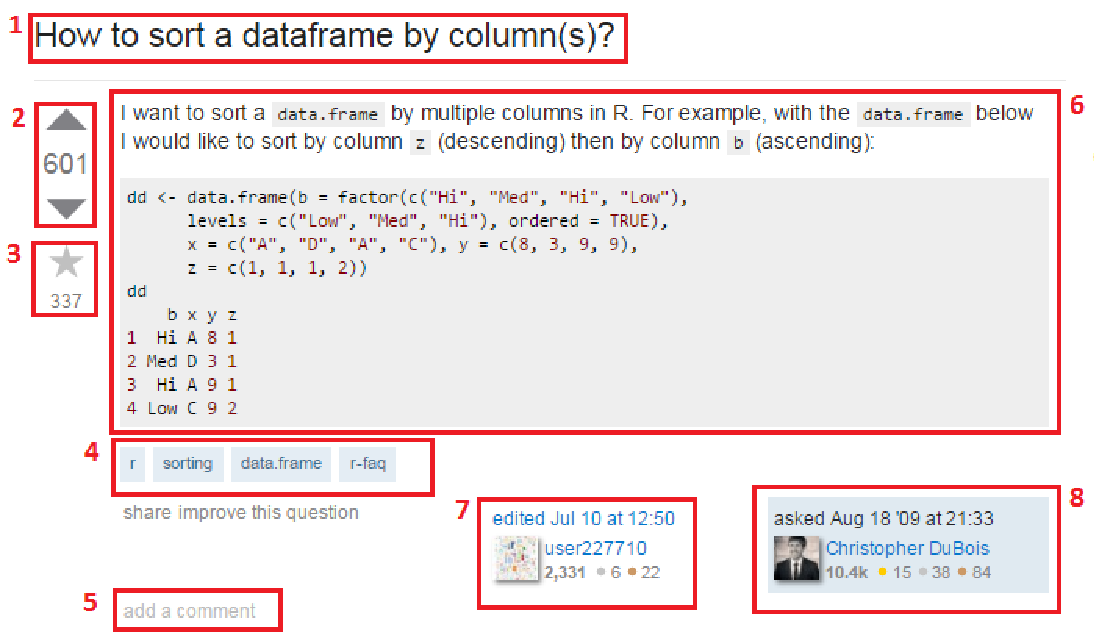
\includegraphics[width=\columnwidth]{Figures/SOInterface_A}
%   \caption{Stack Overflow interface [Question section]}
%   \label{fig:SOInterface_A}
%   \end{figure}

%   Stack Overflow's interface is rich with information. Figures \ref{fig:SOInterface_A} and \ref{fig:SOInterface_B} depict the interface separated into two sections. Figure \ref{fig:SOInterface_A} describes the post in relation to the \textit{question}.
%   The elements are numbered from 1 to 8, and are described as follows:
%   (1) title of the question;
%   (2) number of votes for the question, as well as two arrow buttons to vote up (positive) or down (negative);
%   (3) a star button to mark the question as a favourite and the number of users who have done it;
%   (4) tags applied to the question;
%   (5) a button to add a short, text-based comment to the question;
%   (6) body of the question which might contain, along with the description, other aids such as images, source code, examples, and links;
%   (7) last user that edited the question along with their reputation points;.
%   and (8) information of the user who posted the question, including alias, silver and copper badges, and the date of the posted question.

%   \begin{figure}[!htb]
%   \centering
%   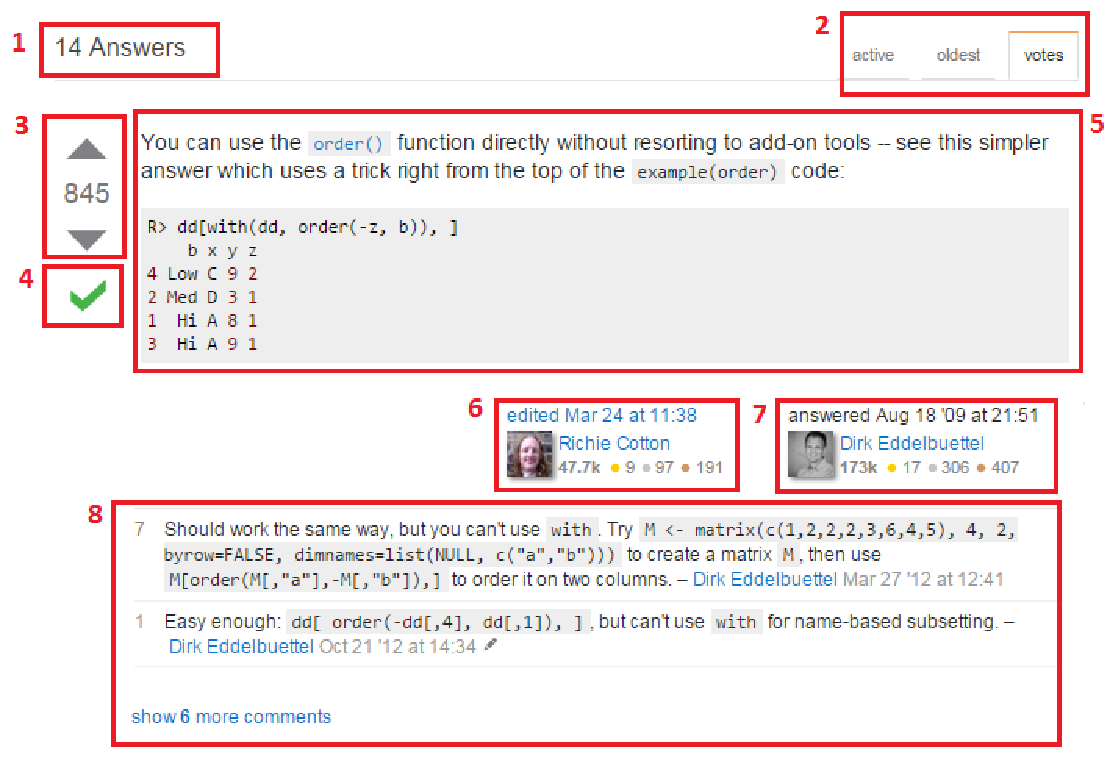
\includegraphics[width=\columnwidth]{Figures/SOInterface_B}
%   \caption{Stack Overflow interface [Answer Section]}
%   \label{fig:SOInterface_B}
%   \end{figure}

%   Figure \ref{fig:SOInterface_B} shows the post in relation to the \textit{answer} located below the question in the interface.
%   The elements are numbered 1 to 8, and are described as follows:
%   (1) number of answers provided to the question;
%   (2) sorting buttons to display the answers by latest activity, oldest first, or most recent first;
%   (3) number of votes for the answer, as well as two buttons (up and down arrows) to allow users to vote up (positive) or down (negative);
%   (4) a check mark to indicate that the owner of the question marked the answer as the solution to the question;
%   (5) body of the answer which might contain, along with the proposed solution, other aids such as images, source code, examples, and links;
%   (6) last user that edited the question along with their reputation points;
%   (7) information about the user who posted the question, including alias, silver and copper badges, and the date of the posted question;
%   and (8) comments to the answer, which are fairly short and limited to include only text.

    The adoption of social media has occurred at a much faster rate than any previous communication technology \cite{Chui2012}.
    In the last decade, Stack Overflow has become the most popular media channel for answering software development related questions, nearly replacing previous methods of communication that accomplished the same objective~\cite{Vasilescu2014c}.
    %<<
%   Figure~\ref{fig:VasilescuFA1-1} shows the number of questions asked each month on Stack Overflow, Cross Validate and the R-help mailing list, and Figure~\ref{fig:VasilescuFA1-2} shows the number of questions answered on the R-help mailing list (after September 2008) and Stack Exchange each month.
    %>>
    Despite Stack Overflow's advantages over Q\&A mailing lists such as the R-help (i.e., gamification environment and rich visual user interface), there are still many users who prefer the latter.
    We will learn the way programmers use Stack Overflow and the R-help mailing list to gain and share knowledge.

%   \begin{figure}
%       \centering
%       \begin{subfigure}[b]{\columnwidth}
%         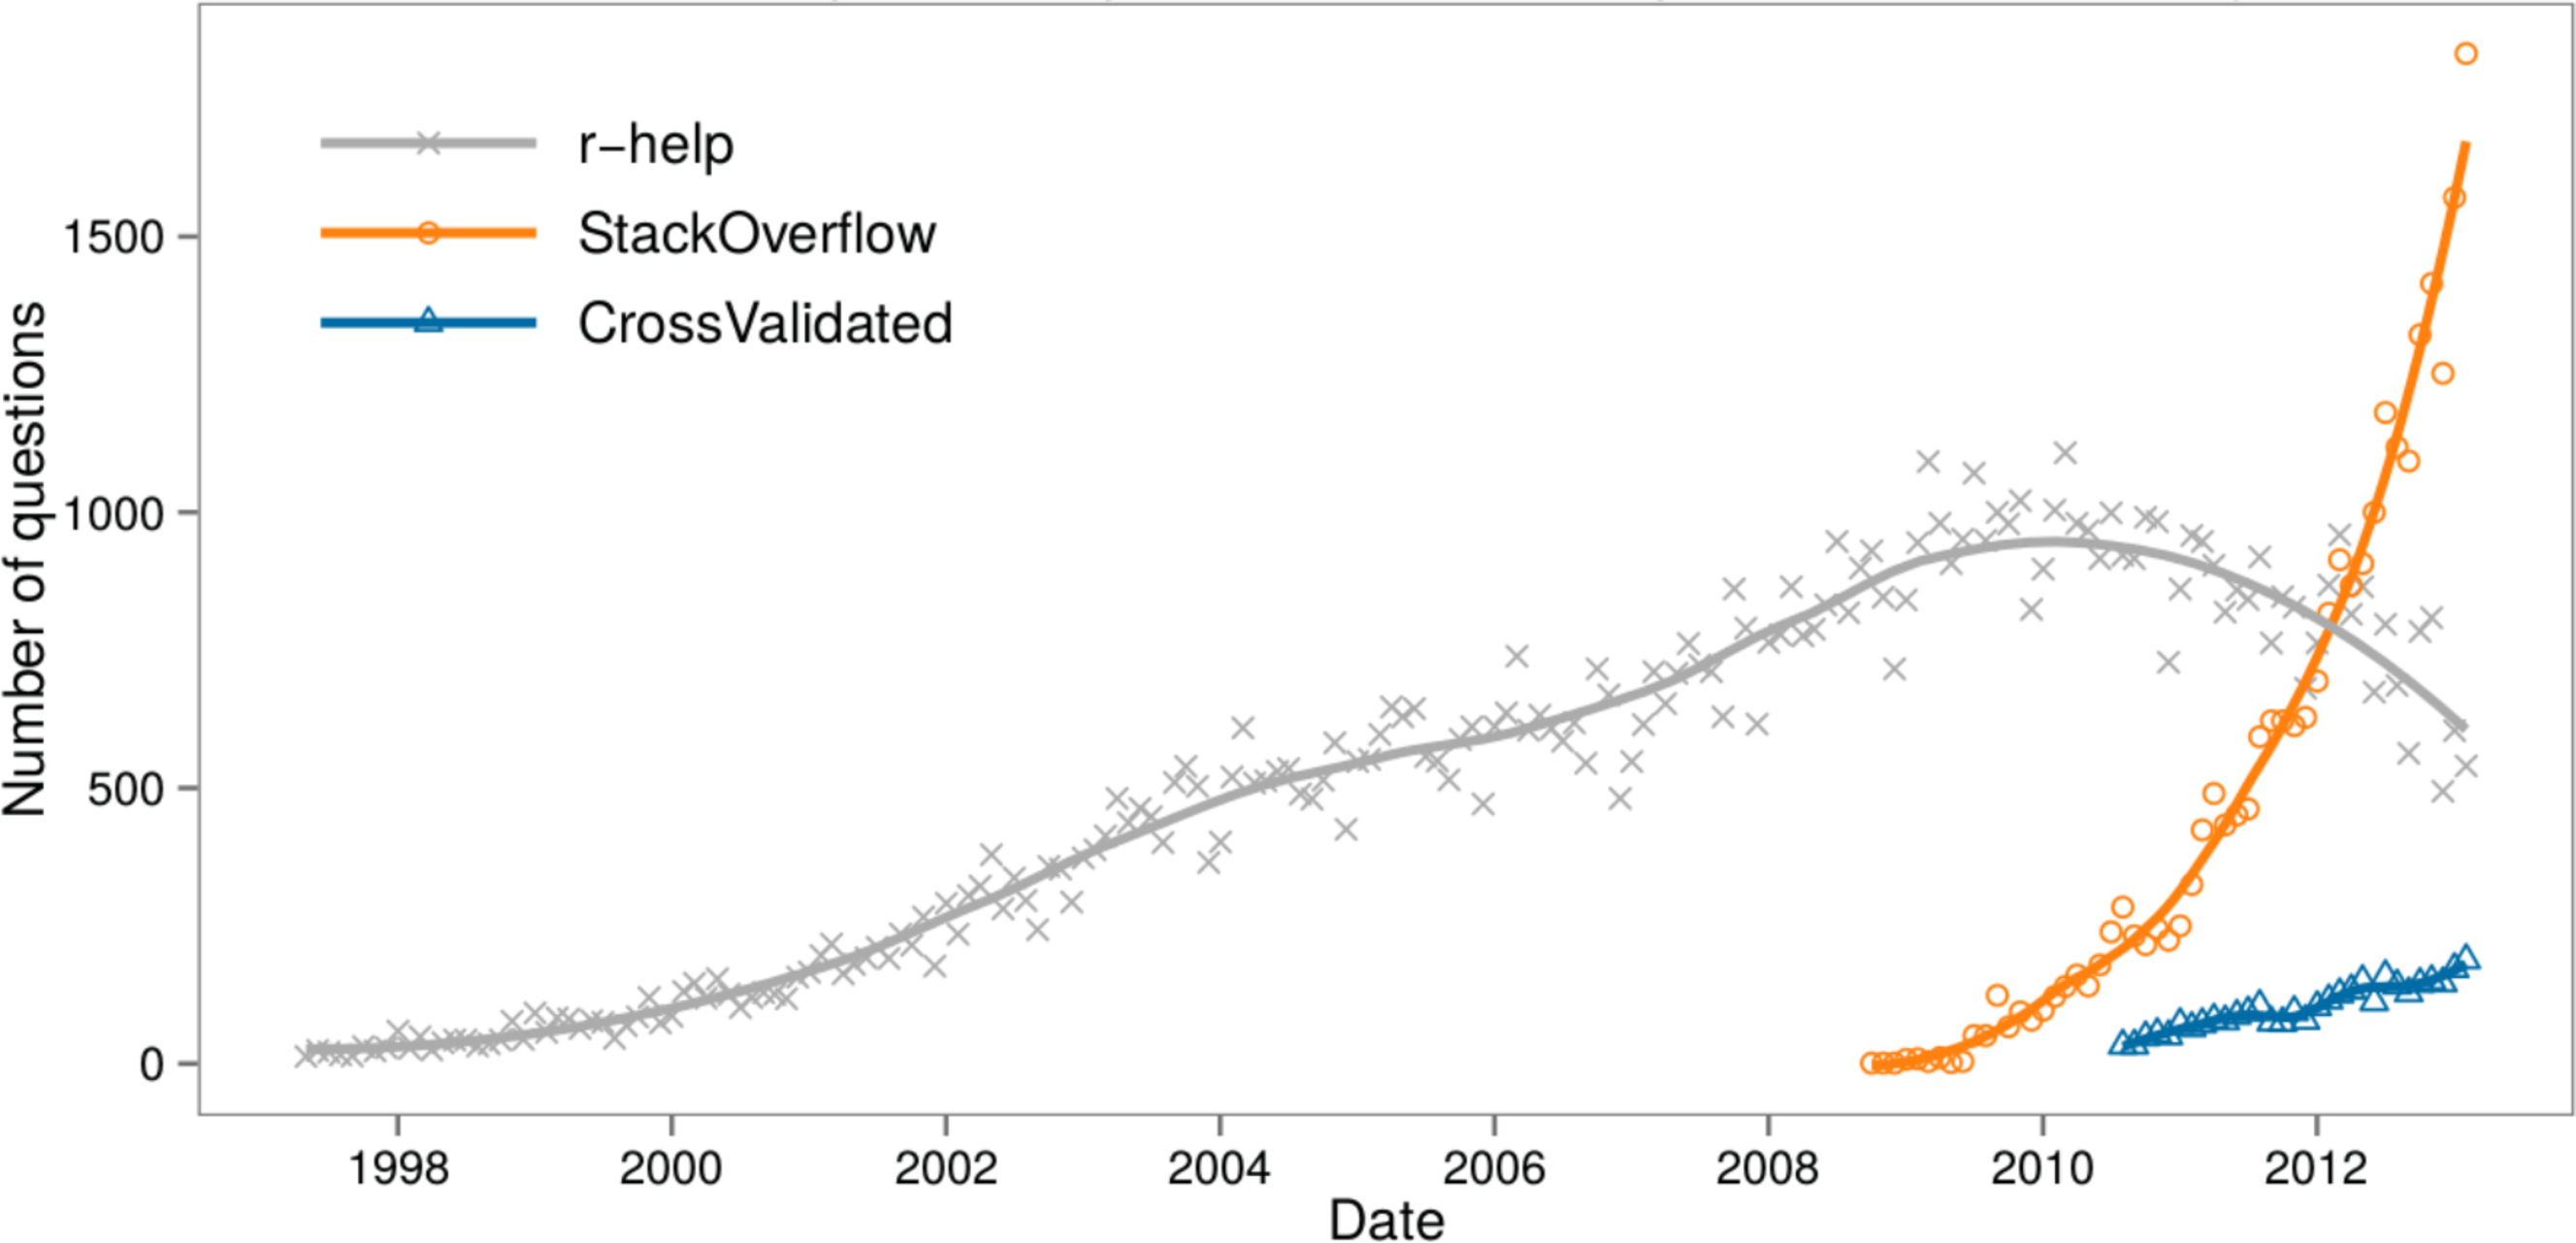
\includegraphics[width=\columnwidth]{Figures/VasilescuFA1}
%          \caption{Questions asked (threads started) per month on R-help and Stack Exchange (Stack Overflow and Cross Validated).}
%         \label{fig:VasilescuFA1-1}
%        \end{subfigure}
%       \begin{subfigure}[b]{\columnwidth}
%         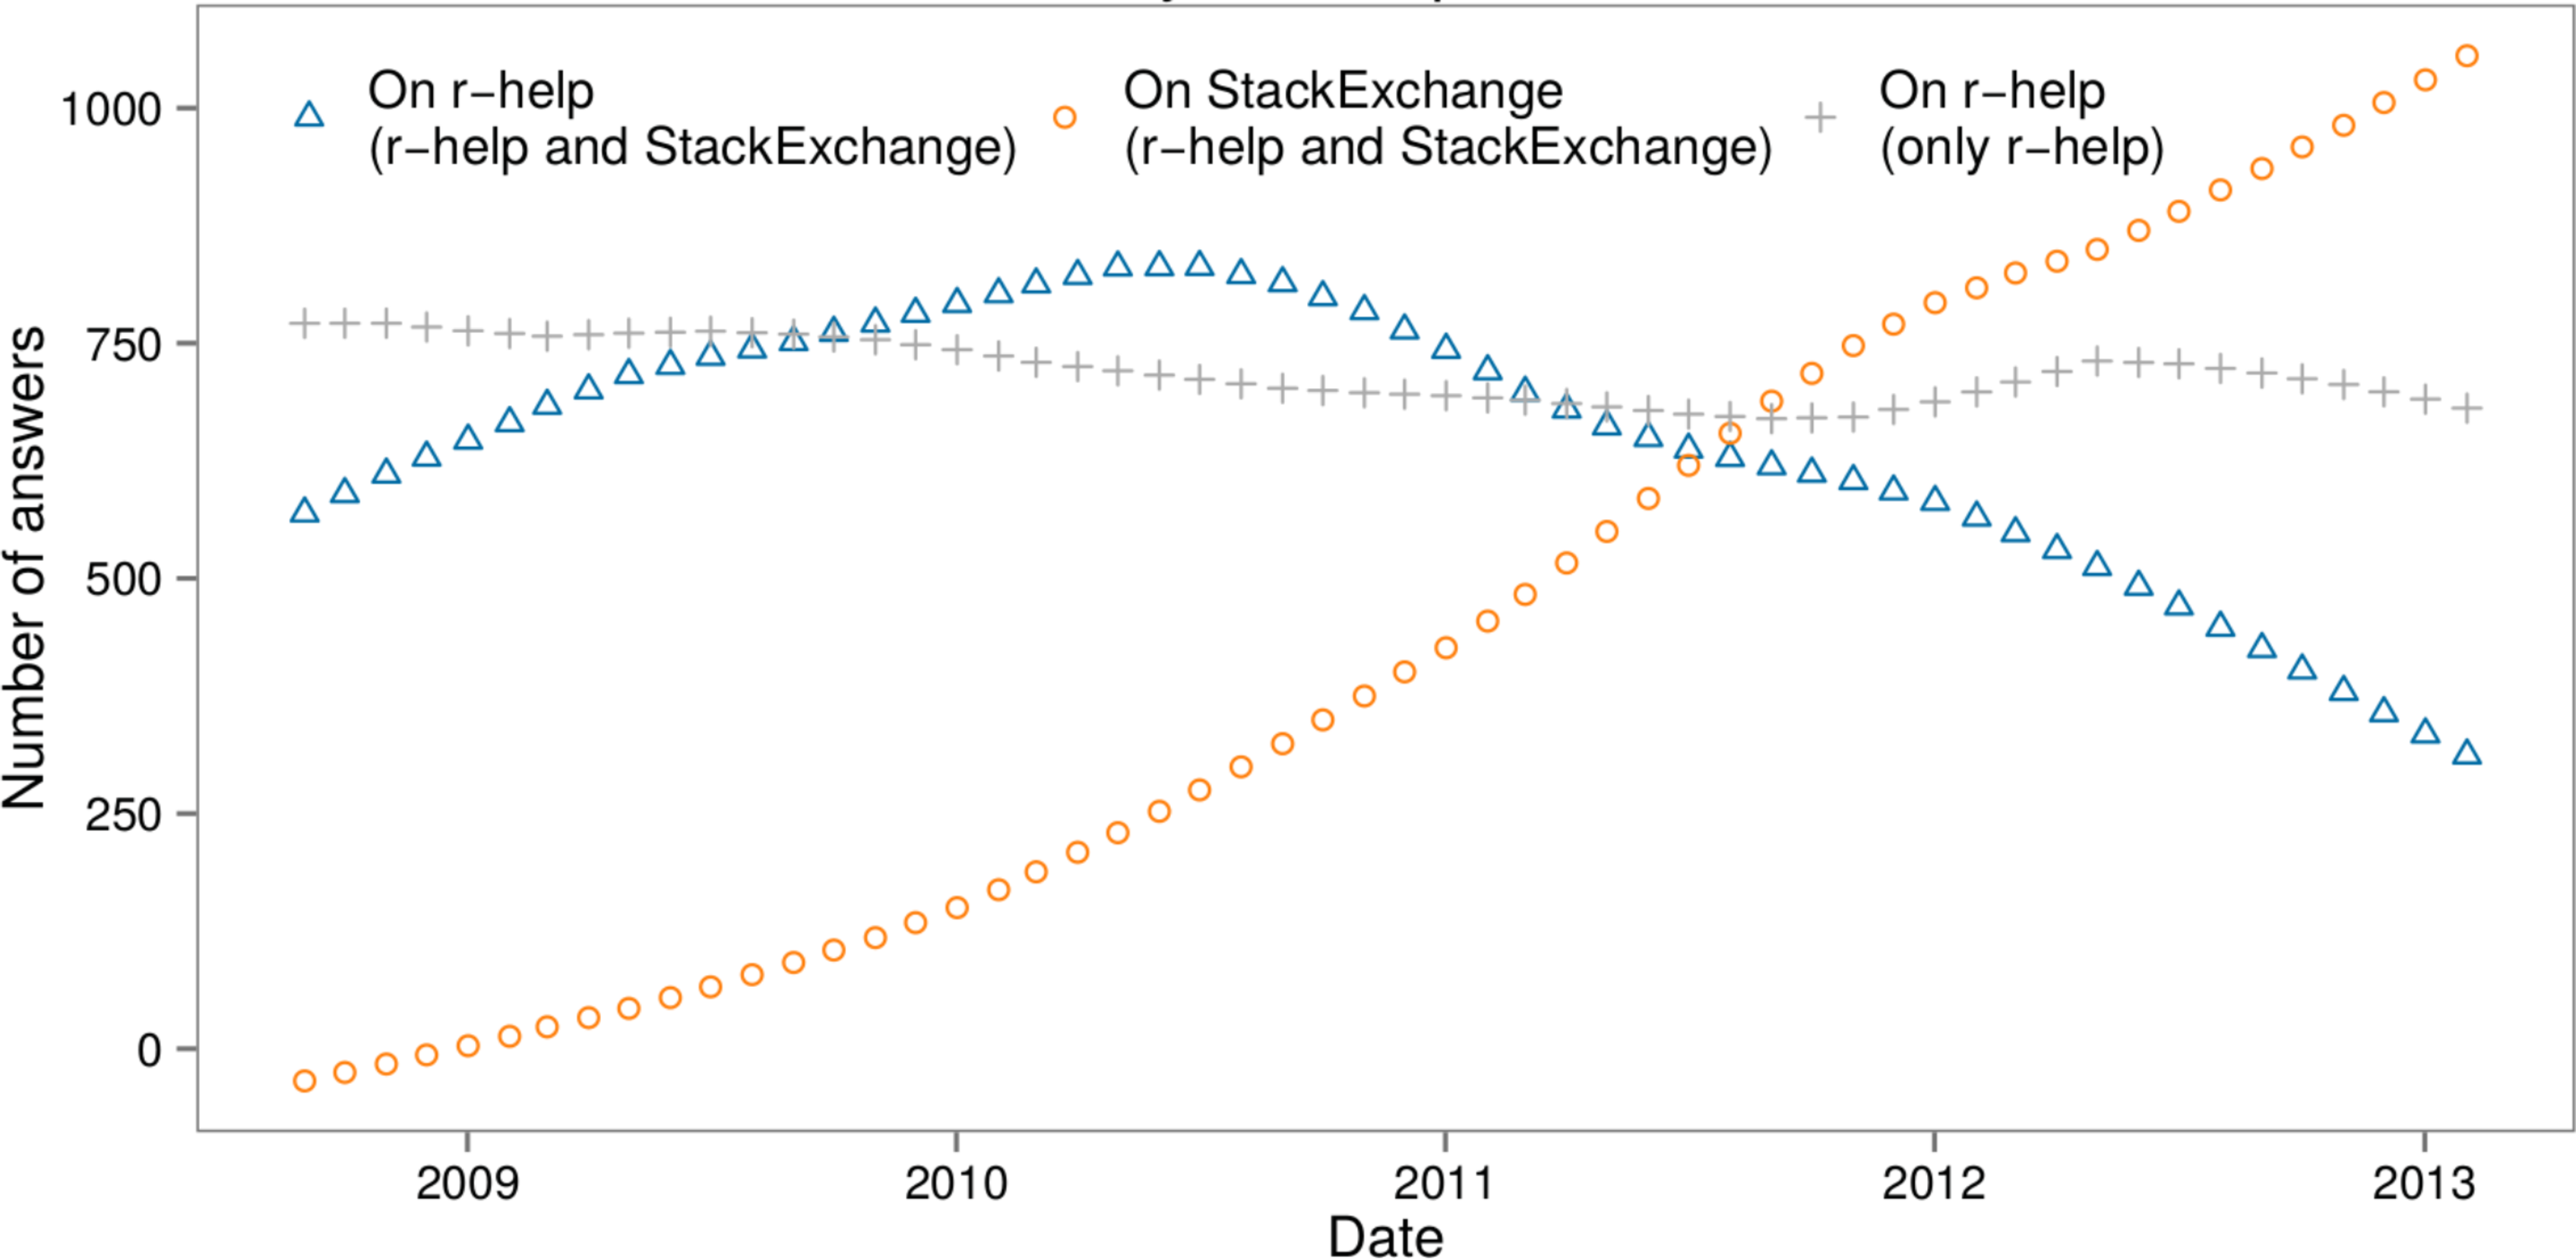
\includegraphics[width=\columnwidth]{Figures/VasilescuFA2}
%          \caption{Questions answered on R-help mailing list (after September 2008) and Stack Exchange per month: participants exclusive to the mailing list versus those also active on Stack Exchange.}
%         \label{fig:VasilescuFA1-2}
%        \end{subfigure}
%       \caption{Number of questions asked and answered~\cite{Vasilescu2014c}.}
%       \label{fig:VasilescuFA1}
%   \end{figure}